\newpage
\setcounter{figure}{0}

\section{Rezultati} % (fold)
\label{sec:Rezultati}

Tijekom izrade diplomskog rada snimljeno je šest scena upotrebom
programa RGBDSlam i iz tih snimaka (slika~\ref{fig:01-all.png}) 
izgrađeni su 3D modeli objekata i scena pomoću programa
\texttt{mesh-reconstruction}. Sve snimke i izrađeni modeli nalaze se na
priloženom DVDu. U ovom poglavlju su prikazani rezultati izgradnje i
ispitana je funkcionalnost izgradnje 3D modela scena pomoću 3D kamere.
Za ispitivanje funkcionalnosti metode odabrane su tri scene:
\texttt{etfos-ured-2013-07-30}, \texttt{etfos-hol-2013-11-20},
\texttt{etfos-hodnik-11-27}. Prije prikaza rezultata potrebno je
istaknuti nekoliko problema odnosno ograničenja ove metode.

Proces snimanja scena RGBDSlam programom odnosno stjecanje oblaka je
obilježen s par problema i ograničenja. Program se nekoliko puta srušio
tijekom snimanja te su snimljeni podaci bili izgubljeni. Ustanovljeno je
da se RBGSlam sruši ako je u ručnom načinu rada te se pritisne tipka
\texttt{Backspace} koja bi trebala obrisati zadnju uzetu sliku. Također
prilikom snimanja pažljivo je odabran "put" snimanja svake scene kako
bih program uspješno mogao spariti značajke s prethodnim slikama te na
kraju zatvoriti petlju i ispraviti akumulirane greške. Unatoč tome kao
što se vidi među rezultatima na nekim mjestima program nije uspješno
spario značajke niti je zatvorio petlju.

Proces izgradnje 3D modela scene \texttt{mesh-reconstruction} programom
obilježen je ograničenjem Poisson algoritma. Algoritam spaja odnosno
popunjava regije/rupe bez točaka u modelu. Isto tako implementacija
algoritma u PCL biblioteci ne uzima u obzir informaciju o boji prilikom
izgradnje modela.

\begin{figure}[h]
\centering
\includegraphics[scale=0.20]{figures/01-all-pcd.png}
\caption{Prikaz svih snimljenih scena}
\label{fig:01-all.png}
\end{figure}

\newpage
\subsection{Prikaz izgrađenih modela scena i objekata} % (fold)
\label{sub:Prikaz izgradenih modela scena i objekata}

\textbf{Snimka: Etfos ured 2013-07-30} 

\begin{figure}[h]
\centering
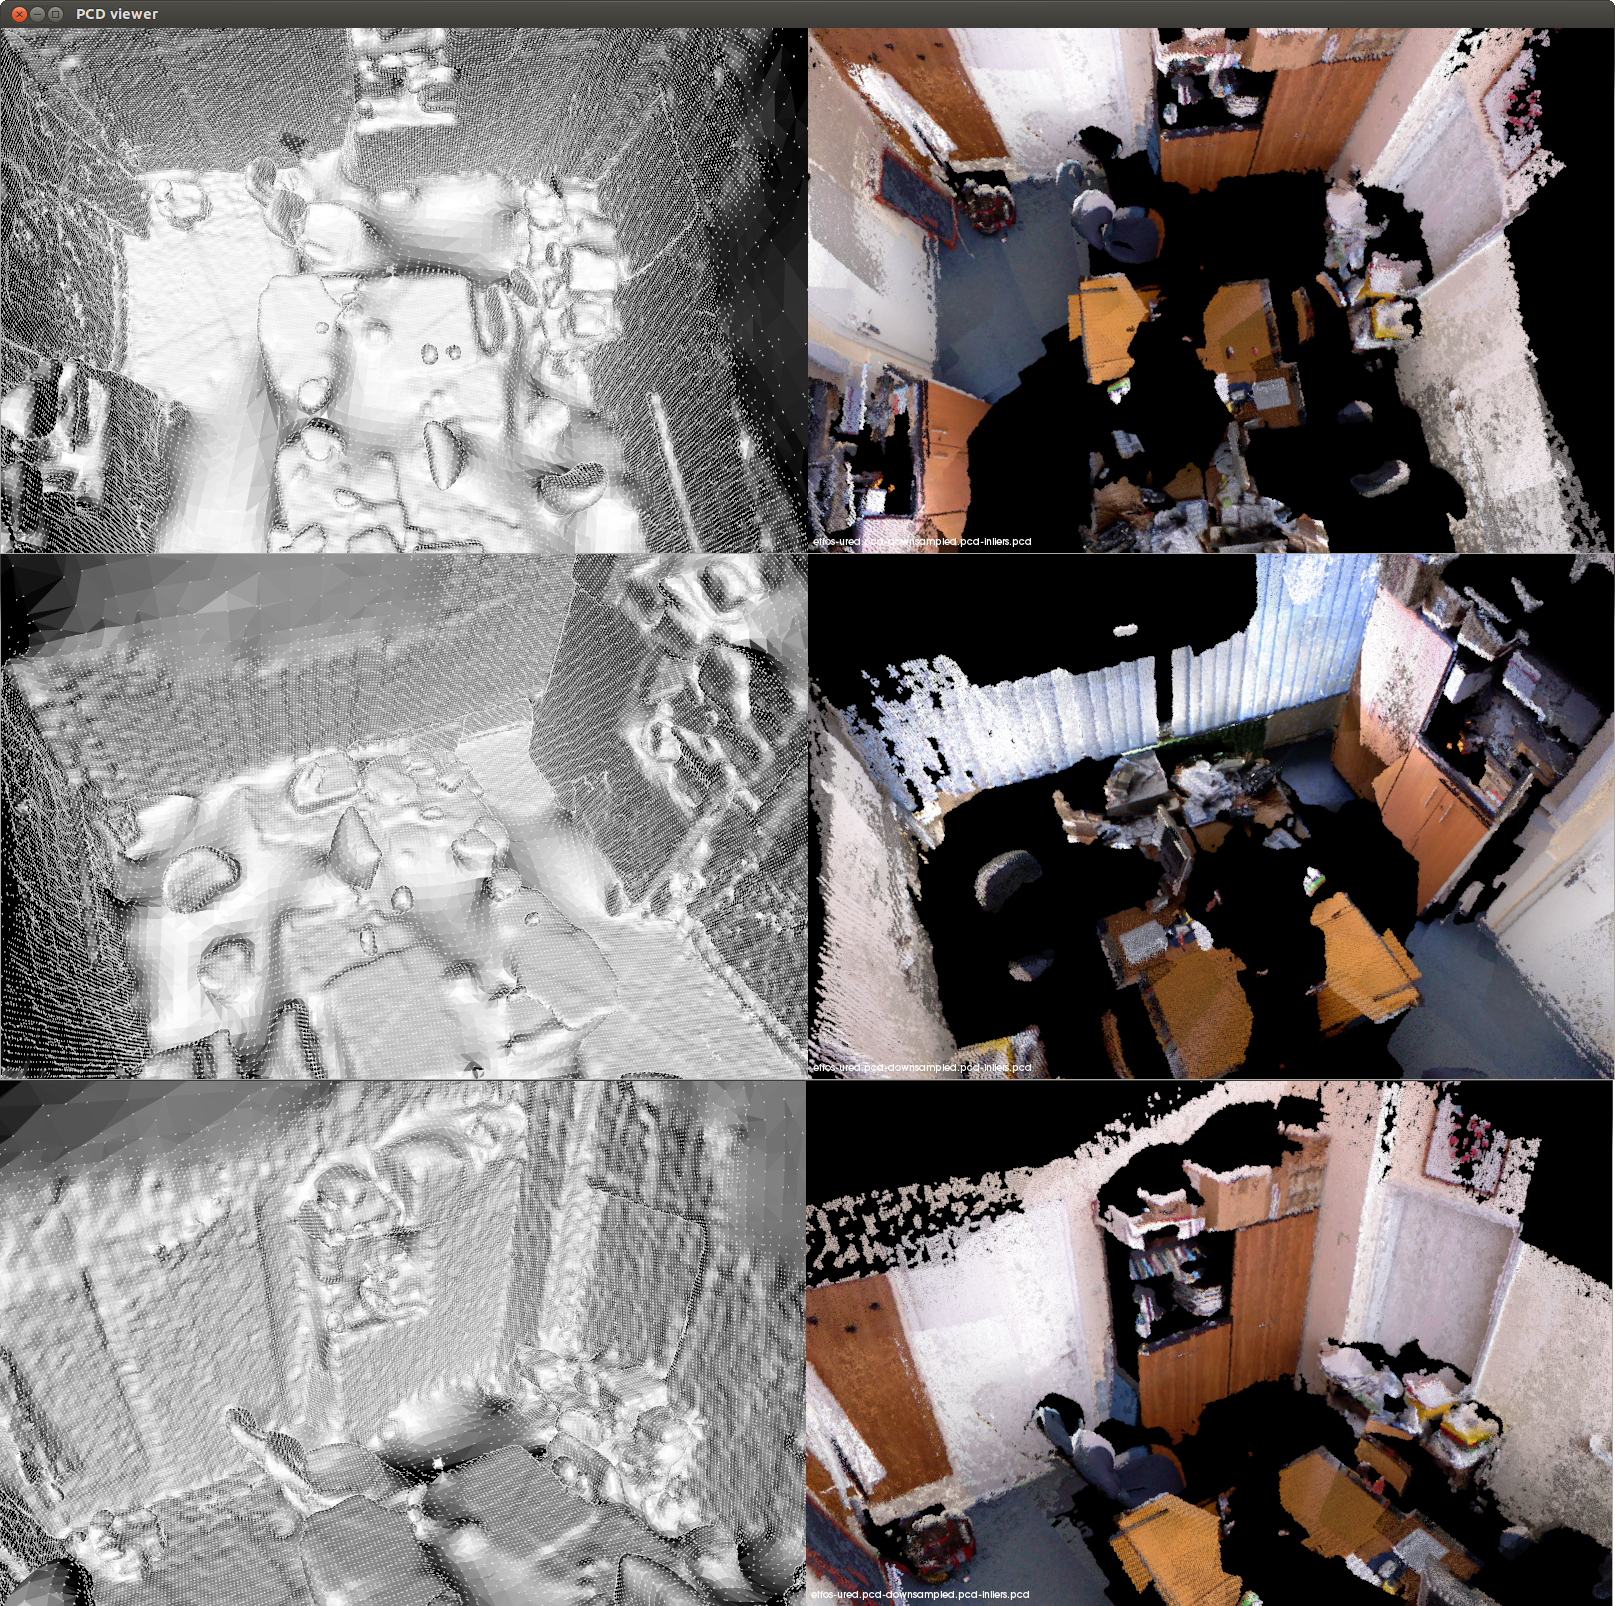
\includegraphics[scale=0.25]{figures/02-etfos-ured-vtk-pcd-all.png}
\caption{Prikaz izrađenog modela i snimljenog oblaka točaka}
\label{fig:02-etfos-ured-vtk-pcd.png}
\end{figure}

% subsection Prikaz izgrađenih modela scena i objekata (end)

% section Rezultati (end)

